\documentclass{article}

\usepackage{amsmath}
\usepackage{graphicx}

\title{Extracting Information from Star Forming Clumps: Temperature, Mass and Luminosity}
\date{2020-04-14}
\author{Morgan Langford}

\begin{document}

\pagenumbering{gobble}
\maketitle
\newpage
\pagenumbering{arabic}

\tableofcontents
\newpage

\section{Introduction}
\subsection{Star Formation}
\paragraph{}

The interstellar medium (ISM), the space between the stars, has four components: matter, in the form of dust and gas; electromagnetic radiation; gravitational fields and magnetic fields (Kay, Palen, Smith, \& Blumenthal, 2013). It has a chemical composition of $~90\%$ Hydrogen, $~10\%$ Helium and only $~0.1\%$ more massive elements (Kay et al., 2013). $~99\%$ of interstellar matter is gaseous and it has an average density of $0.1 atoms/cm^3$. To give some point of reference, the air we breathe on Earth is about $2.7 x 10^{19} atoms/cm^3$ and the best vacuum we can create is $10^{10} atoms/cm^3$. 

\begin{figure}[h!]
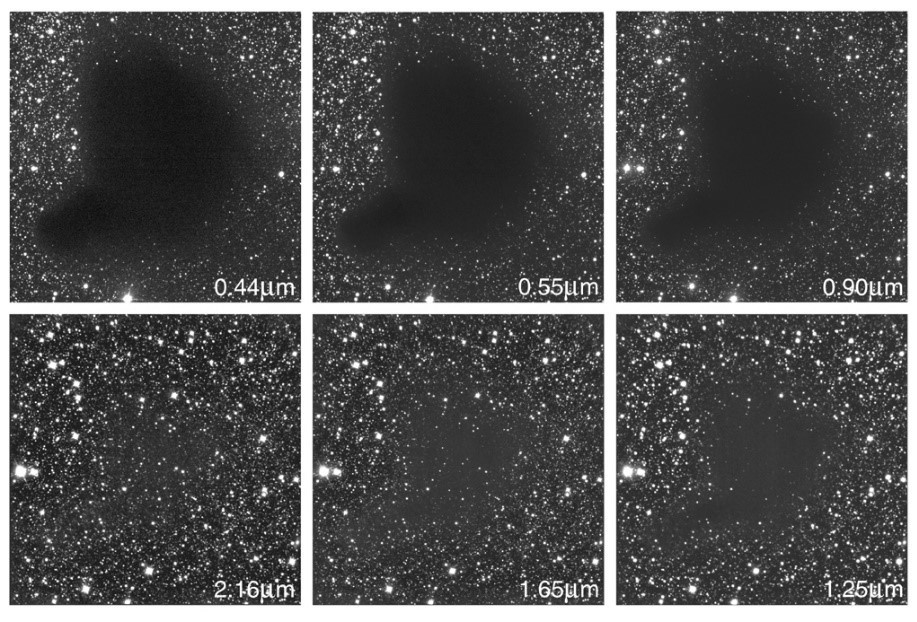
\includegraphics[width=\linewidth]{dust.jpg}
\caption{Images of the same cloud, taken at different wavelengths displaying 'interstellar extinction' (Walter, 1999)}
\label{fig:dust1}
\end{figure}

Interstellar dust makes up approximately $1\%$ of the material in the ISM. In size, it ranges from the size of a large molecule to $~300 nm$ across (Kay et al., 2013). Don’t be fooled by its size, however, as it is extremely good at blocking out light. This is known as interstellar extinction. It best blocks out light which has a wavelength about the size of the dust grain, meaning short wavelengths are absorbed or scattered whereas long wavelengths pass through, uninhibited (Bergin \& Tafalla, 2007). This effect is displayed in Figure \ref{fig:dust1}, showing the cloud quite visible at $0.44 µm$ and almost invisible at $2.16 µm$, suggesting a large number of the dust grains are around $0.44 µm$ in size. 
\paragraph{}
Interstellar clouds have an average temperature of $~100 K$. Wien’s Displacement Law calculates the peak of the black body radiation to be at $2.90x10^{-5} m$, or $29.0 nm$. They are composed of mostly neutral atomic Hydrogen (Bergin \& Tafalla, 2007). They are relatively dense, at a density of $1 – 100 atoms/cm^3$ (Kay et al., 2013). Only in the densest clouds can molecules exist; these are known as molecular clouds. They are approximately $10 K$, cold and dense. They have a density of $100 – 1000 atoms/cm^3$ and they range between $½$ a light year to $1000$ light years in size. 
\paragraph{}
Cold Dark Clouds (CDCs) are where molecular clouds are formed; they contain both atomic and molecular gas and are a density and temperature intermediate between the atomic ISM and molecular clouds (East Asian Observatory, n.d.-b). Only about $¼$ of the mass of the ISM is in molecular form and most of it is found in giant molecular clouds (GMCs) (Molinari et al., 2010). These GMCs contain clumps which, in turn, contain cores and it is within these cores that a star is formed (Williams, Blitz, \& McKee, 1999). 
\paragraph{}
Stellar nurseries are known as the ‘cradles’ of star formation (Kay et al., 2013). These interstellar clouds are massive enough to have self-gravity. If an interstellar cloud is massive, dense and cool enough, the self-gravity is enough to overpower the internal gas pressure pressing against it, and the cloud collapses under its own weight (Jeans, 1902).
\paragraph{}
Because molecular clouds are never uniform, some areas collapse faster at an accelerated rate, due to the inverse square law of gravity (Kay et al., 2013). Self-gravity becomes stronger in these areas and these are what form molecular cores. Due to the angular momentum of the cloud, it forms a flat, rotating disk, also known as an accretion disk with a protostar at the center (Kay et al., 2013). 
\paragraph{}
Within the protostar, gravitational energy is converted to thermal energy, increasing its temperature (Kay et al., 2013). The protostar is 100x the size of the sun, with a surface area of tens of thousands of times larger making it 1000x more luminous. There are still no nuclear reactions. 
\paragraph{}
The forces acting on the protostar are still relatively balanced; the hot-gas pressure outward roughly equals the self-gravity pulling inward (Kay et al., 2013). This is constantly changing as material continuously falls onto the protostar. The increased gravitational pull increases the internal pressure. The increased gravity increases the internal pressure, and the protostar keeps growing hotter until, finally, Hydrogen fusion happens!

\section{Objective}
\paragraph{}

The first part of this project is to extract the fluxes from star forming clumps using software and photometry. For the main part of the project, the flux has already been extracted using two computer algorithms: ‘CUTEX: CUrvature Thresholding EXtractor’ (Molinary et al. 2010) and FellWalker (Berry 2015). This exercise gives a better understanding of the background of the data.
\paragraph{}
The main part of the project is to extract the temperature, mass and luminosity of the given clumps. This is done via a Spectral Energy Distribution (SED) fitting algorithm, where an SED is a plot of the energy emitted by an object as a function of its wavelengths. 

\section{Observation}
\subsection{Herschel}
\paragraph{}

The Herschel Space Observatory (HSO) was set to discover information about the early universe (Herschel, 2013). It detected radiation at far infrared and submillimeter wavelengths and was able to then observe dust in the ISM which was, otherwise, invisible. One of Herschel’s purposes was to observe interstellar clouds.
\paragraph{}
The Herschel infrared Galactic Plane Survey (Hi-GAL) was a photometric survey which mapped a two-degree wide strip at five wavelengths with its two cameras, PACS and SPIRE (Molinari et al., 2010). PACS collected data at 70 and 170 µm and SPIRE did so at 250, 350 and 500 µm. 

\subsection{James Clerk Maxwell Telescope}
\paragraph{}

The James Clerk Maxwell Telescope (JCMT) is a ground-based telescope based at Mauna Kea Observatory in Hawaii, US (East Asian Observatory, n.d.-a). Observatories like this one are built in dry, high-altitude regions like Mauna Kea for three reasons: there is less atmosphere, the lack of water vapor causes less distortion and there is less atmospheric turbulence due to lack of pollution. It is the largest astronomical telescope in the world that is designed to operate in the submillimeter wavelength part of the spectrum. 
\paragraph{}
The objective of the JCMT Galactic Plane Survey was to get a full survey of star-formation activity in the plane of the Galaxy which is observable from JCMT (East Asian Observatory, n.d.-b). Two of the four main goals were to observe the star-forming content of molecular clouds, Cold Dark Clouds and the formation of molecular clouds. Arrays like SCUBA have made it possible to map the thermal emission of cold dust from dark clouds (Bergin \& Tafalla, 2007).

\subsection{Spectral Energy Distributions}
\paragraph{}

Though stars and protostars have the characteristics of a blackbody, interstellar dust has those of a gray body (Dall’Oglio, Morgante, Pizzo, Valenziano, \& Merluzzi, 1995). Therefore, a modified Plank function is required to describe the radiation it emits. This is known as the radiative transfer equation.

\begin{center}
$F_v={[(1-e^{-\tau_c } ) B_v T_c \Omega_c ]_c}$
\end{center}

\paragraph{}
Spectral Energy Distributions (SEDs) are a plot of the radiative flux against the wavelength. It is this SED from which the temperature, mass and luminosity may be extracted. 

\section{Solution}
\subsection{Timeline}

\begin{figure}[h!]
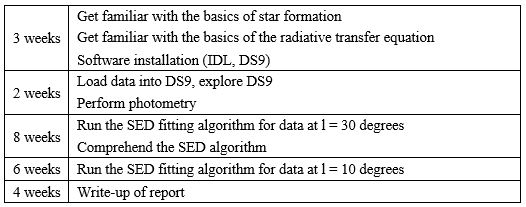
\includegraphics[width=\linewidth]{timeline.jpg}
\caption{Timeline}
\label{fig:timeline1}
\end{figure}

\subsection{Software Required}
\paragraph{}
SAOImage DS9 (DS9)

\begin{itemize}
\item DS9 is an astronomical imaging and data visualization application
\item This will be used to perform photometry on the given data
\item Cost: \$0
\end{itemize}

\paragraph{}
Harris Geospatial - IDL (Interactive Data Language)

\begin{itemize}
\item IDL is a scientific programming language is used to visualize complex data
\item This will be used to run the algorithm
\item Cost: \$80 for student subscription
\end{itemize}

\subsection{Expected Outcome}
\paragraph{}
To have used the SED fitting algorithm to extract the physical condition (i.e. the temperature, mass and luminosity) of the star forming region, including all the identified clumps.  

\section{SWOT Analysis}

\subsection{Strengths}

\begin{itemize}
\item I am working with a consulting professor, Professor Kianoosh Tahani, PhD. He is an astrophysicist who has worked on a similar project previously.
\item I have experience in programming and in Astronomy
\item The SED fitting algorithm is already written 
\item The flux has already been extracted
\end{itemize}

\subsection{Weaknesses}

\begin{itemize}
\item I am unfamiliar with IDL, the programming language.
\item I did not write the algorithm which makes debugging it difficult.
\item The algorithm was written for Linux; it needs to be modified for Windows. 
\end{itemize}


\subsection{Opportunities}
\paragraph{}
There is a further project related to this one that I can do if I have time to get to it but no spoilers.

\subsection{Threats}
\paragraph{}
There is a chance that the algorithm will not work on Windows and will have to be partially rewritten. As I do not have experience with IDL, this could not be done by me. 
\paragraph{}
If it proves hard to get the IDL license, there is no other option for running the algorithm. I will have to be approved for the student licence because the commercial license is well out of the budget. 
\paragraph{}
All the final data will be kept in one very large file so it must be backed up in multiple places including the cloud for fear of losing it. 

\begin{appendix}
\listoffigures
\end{appendix}

\newpage

\section{References}
\begin{figure}[h!]
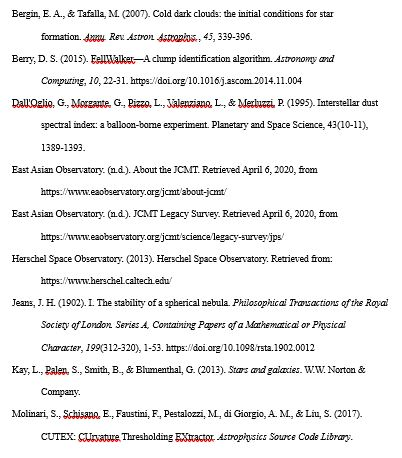
\includegraphics[width=\linewidth]{refspage1.jpg}
\end{figure}

\begin{figure}[t!]
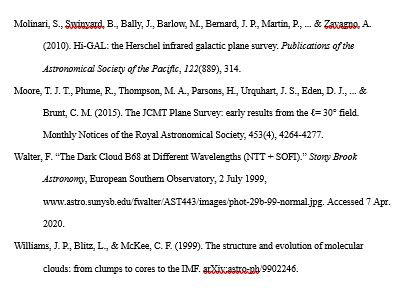
\includegraphics[width=\linewidth]{refspage2.jpg}
\end{figure}

\end{document}